\chapter{A energia das reações: combustão e energias de ligação}\label{ch:g11:reaction-energy}

Rompa o lacre de um aquecedor de mãos e, um minuto depois, ele está
quente demais para ser segurado por muito tempo; aperte uma compressa
fria instantânea e ela gela um tornozelo torcido; um ônibus urbano roda
o dia inteiro com hidrogênio e só deixa vapor de água atrás de si. As
\omterm{def:g5:irreversible-changes:chemical-change}{transformações químicas} não só transformam substâncias em outras: elas
liberam energia, ou a absorvem. De onde vem essa energia, e quanto dela
um \omterm{def:g4:what-a-fire-needs:fuel}{combustível} pode dar?

\begin{recall}
Numa \omterm{def:g8:combustion-and-fuels:complete}{combustão completa}, um \omterm{def:g4:what-a-fire-needs:fuel}{combustível} feito de carbono e hidrogênio
\omterm{def:g4:what-a-fire-needs:burning}{queima} no gás oxigênio e dá dióxido de carbono e água
(\cref{ch:g8:combustion-and-fuels}). Uma \omterm{def:g10:lewis-and-shape:covalent-bond}{ligação covalente} é um par de
\omterm{def:g9:inside-the-atom:nucleus}{elétrons} compartilhado; as \omterm{def:g10:lewis-and-shape:lewis-structure}{estruturas de Lewis} mostram todas as ligações
de uma \omterm{def:g7:atoms-and-molecules:molecule}{molécula} (\cref{ch:g10:lewis-and-shape}). A \omterm{def:g10:the-mole:amount}{quantidade de matéria}
é contada em \omterm{def:g10:the-mole:amount}{mols} (\cref{ch:g10:the-mole}).
\end{recall}

\begin{omfigure}
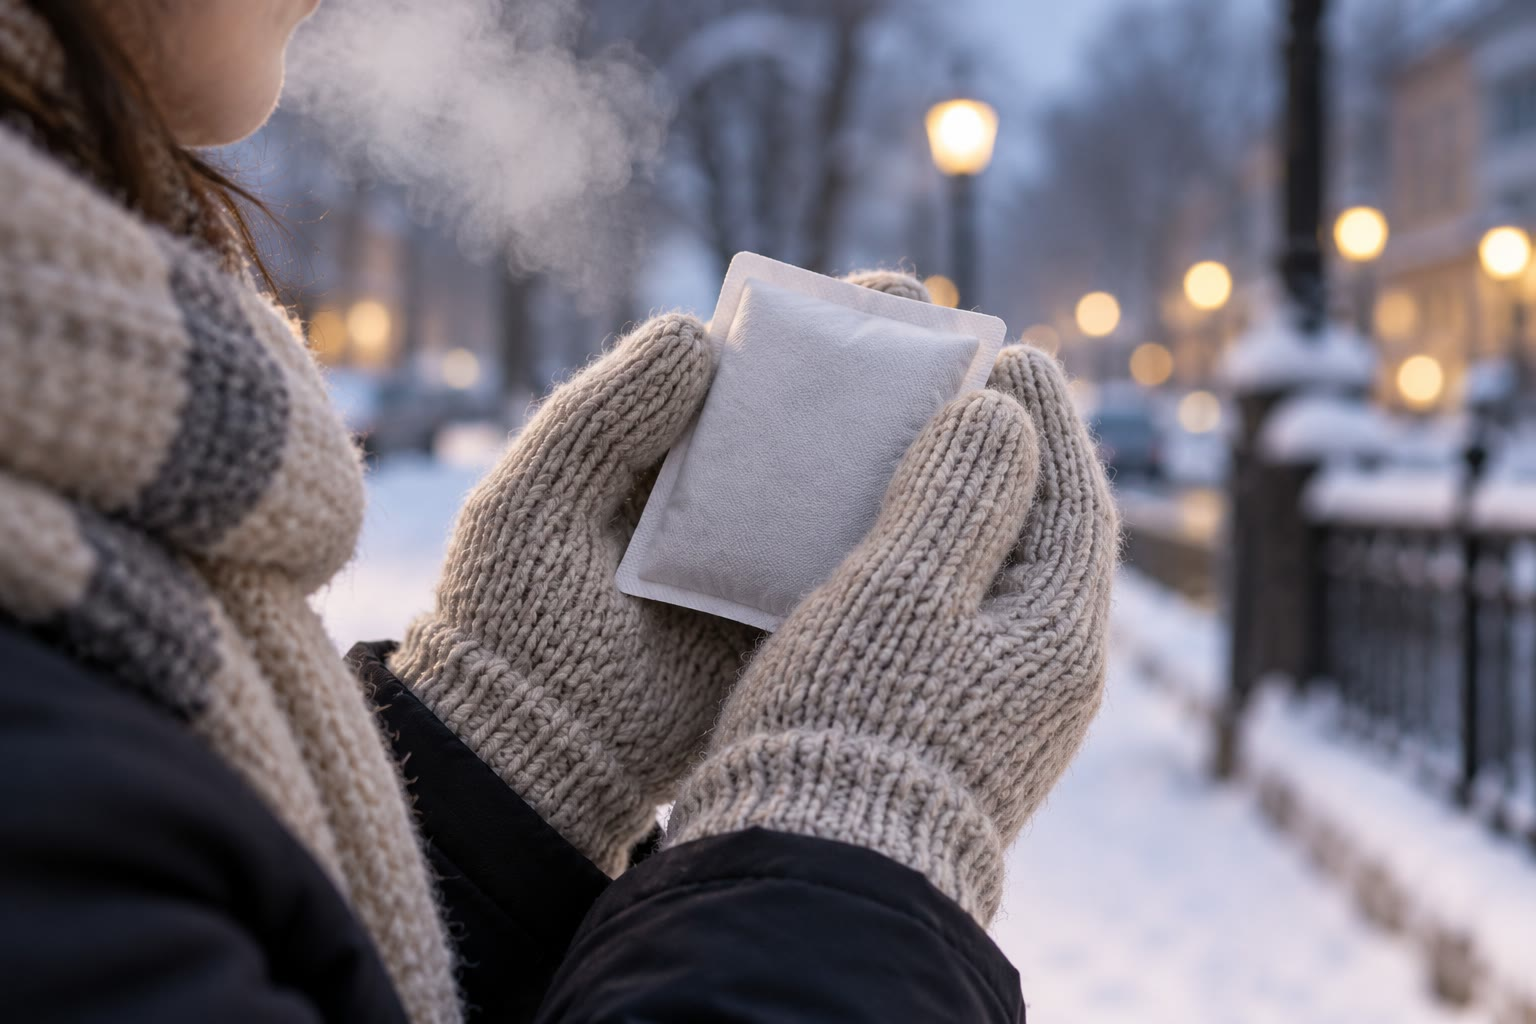
\includegraphics[width=0.45\linewidth]{images/book1/ai/g11-hand-warmers.jpg}

{\small Um aquecedor de mãos: uma reação dentro do saquinho libera
calor.}
\end{omfigure}

\section{Transformações exotérmicas e endotérmicas}

\begin{definition}[Exotérmica, endotérmica]\label{def:g11:reaction-energy:exothermic}
Uma transformação é \emph{exotérmica}\index{exotermica@exotérmica} se ela libera
energia para a sua vizinhança, em geral na forma de calor: a vizinhança
esquenta. Ela é \emph{endotérmica}\index{endotermica@endotérmica} se ela absorve
energia da sua vizinhança: a vizinhança esfria, ou a transformação
precisa de aquecimento para continuar.
\end{definition}

\begin{example}[Quente e frio]\label{ex:g11:reaction-energy:packs}
As \omterm{def:g4:what-a-fire-needs:burning}{combustões} são \omterm{def:g11:reaction-energy:exothermic}{exotérmicas}, e também a reação lenta do ferro em pó
com o gás oxigênio do \omterm{def:g4:air-a-mixture-of-gases:air}{ar} dentro de um aquecedor de mãos. A dissolução do
nitrato de amônio na água, usada nas compressas frias, é \omterm{def:g11:reaction-energy:exothermic}{endotérmica}; e
também a decomposição do calcário em cal virgem e dióxido de carbono,
que só acontece num forno muito quente.
\end{example}

\begin{omfigure}
\begin{tikzpicture}[font=\small]
  \begin{scope}
    \draw[->] (0,0) -- (0,3.2) node[above] {energia};
    \draw[very thick, omDef] (0.5,2.5) -- (2.3,2.5) node[right, text=black] {reagentes};
    \draw[very thick, omProp] (0.5,0.8) -- (2.3,0.8) node[right, text=black] {produtos};
    \draw[->, thick, omThm] (1.4,2.45) -- (1.4,0.85);
    \node[omThm, anchor=west, align=left] at (1.5,1.65) {energia\\ liberada};
    \node[anchor=north] at (1.6,-0.15) {\textbf{exotérmica}};
  \end{scope}
  \begin{scope}[xshift=6cm]
    \draw[->] (0,0) -- (0,3.2) node[above] {energia};
    \draw[very thick, omDef] (0.5,0.8) -- (2.3,0.8) node[right, text=black] {reagentes};
    \draw[very thick, omProp] (0.5,2.5) -- (2.3,2.5) node[right, text=black] {produtos};
    \draw[->, thick, omDef] (1.4,0.85) -- (1.4,2.45);
    \node[omDef, anchor=west, align=left] at (1.5,1.65) {energia\\ absorvida};
    \node[anchor=north] at (1.6,-0.15) {\textbf{endotérmica}};
  \end{scope}
\end{tikzpicture}

{\small Diagramas de energia. Numa reação \omterm{def:g11:reaction-energy:exothermic}{exotérmica}, os produtos têm
menos energia que os \omterm{def:g7:chemical-reactions:reactant}{reagentes}, e a diferença é liberada; numa
\omterm{def:g11:reaction-energy:exothermic}{endotérmica}, eles têm mais, e a diferença tem de ser fornecida.}
\end{omfigure}

\section{A energia liberada por uma combustão}

\begin{definition}[Energia molar de combustão]\label{def:g11:reaction-energy:combustion-energy}
A \emph{energia molar de combustão}\index{energia molar de combustao@energia molar de combustão}
$E_c$ de um \omterm{def:g4:what-a-fire-needs:fuel}{combustível} é a energia liberada pela \omterm{def:g8:combustion-and-fuels:complete}{combustão completa} de
um \omterm{def:g10:the-mole:amount}{mol} dele, em \si{kJ/mol}, com a água formada no estado líquido.
\end{definition}

\begin{proposition}[A energia liberada por $n$ mols]\label{prop:g11:reaction-energy:n-moles}
% ledger: dch:CH4
A \omterm{def:g8:combustion-and-fuels:complete}{combustão completa} de uma quantidade $n$ de \omterm{def:g4:what-a-fire-needs:fuel}{combustível} libera a
energia $Q = n \times E_c$. Para o metano, $E_c = \qty{890.7}{kJ/mol}$:
queimar \qty{1.00}{mol} (\qty{16.0}{g}) dele libera cerca de
\qty{891}{kJ}.
\end{proposition}

\begin{proof}
Cada \omterm{def:g10:the-mole:amount}{mol} de \omterm{def:g4:what-a-fire-needs:fuel}{combustível} queimado libera $E_c$; $n$ \omterm{def:g10:the-mole:amount}{mols} liberam $n$
vezes mais.
\end{proof}

\begin{inthelab}[Aquecer água com uma lamparina a álcool]
% ledger: cp:water
Uma lamparina de etanol é pesada e depois acesa debaixo de uma lata de
\omterm{def:g9:periodic-table-first-look:metal}{metal} com \qty{200}{g} de água e um termômetro dentro. Quando a água
esquentou \qty{25}{\celsius}, a chama é apagada e a lamparina é pesada de
novo: ela perdeu \qty{1.50}{g} de etanol. A energia recebida pela água é
calculada com a fórmula da física $Q = m\, c\, \Delta\theta$, em que
$c = \qty{4.18}{J/(g.\celsius)}$ é o calor específico da água. Ela é
muito menor que a energia que o etanol poderia liberar: boa parte do
calor esquenta o \omterm{def:g4:air-a-mixture-of-gases:air}{ar}, a lata e a lamparina, e uma parte do etanol \omterm{def:g4:what-a-fire-needs:burning}{queima}
de forma incompleta.
\end{inthelab}

\begin{omfigure}
\begin{tikzpicture}[font=\small]
  % spirit burner
  \fill[black!8, draw=black!60] (-0.6,0) rectangle (0.6,0.7);
  \fill[cyan!15] (-0.55,0.05) rectangle (0.55,0.45);
  \fill[black!40] (-0.06,0.7) rectangle (0.06,0.95);
  \fill[orange!70!yellow] (0,0.95) .. controls (-0.25,1.25) and (-0.1,1.6) .. (0,1.85)
    .. controls (0.1,1.6) and (0.25,1.25) .. (0,0.95);
  \fill[yellow!40] (0,1.0) .. controls (-0.1,1.2) and (-0.05,1.4) .. (0,1.5)
    .. controls (0.05,1.4) and (0.1,1.2) .. (0,1.0);
  % tripod and can
  \draw[black!60, line width=1pt] (-1.1,0) -- (-0.9,2.1) (1.1,0) -- (0.9,2.1);
  \draw[black!60, line width=1.2pt] (-1.1,2.1) -- (1.1,2.1);
  \fill[black!15, draw=black!60] (-0.8,2.1) rectangle (0.8,3.7);
  \fill[omWater] (-0.75,2.15) rectangle (0.75,3.3);
  % thermometer
  \pic at (0.35,2.35) {thermometer};
  \draw[omProp, thick, <-] (0.6,0.35) -- (2.0,0.35) node[right, text=black]
    {lamparina a álcool (etanol)};
  \draw[omProp, thick, <-] (0.8,2.9) -- (2.0,2.9) node[right, text=black]
    {lata: \qty{200}{g} de água};
  \draw[omProp, thick, <-] (0.45,5.0) -- (2.0,5.0) node[right, text=black]
    {termômetro};
\end{tikzpicture}

{\small Medir a energia dada por um \omterm{def:g4:what-a-fire-needs:fuel}{combustível}: uma lamparina a álcool
aquece uma lata de água cuja elevação de temperatura é medida.}
\end{omfigure}


\begin{example}[A lamparina em números]\label{ex:g11:reaction-energy:burner}
% ledger: cp:water, dch:C2H5OH, aw:C, aw:H, aw:O
A água recebeu $Q = 200 \times 4.18 \times 25 = \qty{2.09e4}{J}$, isto
é, \qty{20.9}{kJ}. O etanol queimado, \qty{1.50}{g}, corresponde a
$1.50 / 46.0 = \qty{0.0326}{mol}$; com $E_c = \qty{1367.6}{kJ/mol}$, ele
poderia liberar $0.0326 \times 1367.6 = \qty{44.6}{kJ}$. Só
$20.9 / 44.6 \approx \qty{47}{\percent}$ disso chegou à água.
\end{example}

\section{As energias de ligação}

\begin{definition}[Energia de ligação]\label{def:g11:reaction-energy:bond-energy}
A \emph{energia de ligação}\index{energia de ligacao@energia de ligação} de uma \omterm{def:g10:lewis-and-shape:covalent-bond}{ligação
covalente} é a energia necessária para romper um \omterm{def:g10:the-mole:amount}{mol} dessas ligações, com
as \omterm{def:g7:atoms-and-molecules:molecule}{moléculas} e os \omterm{def:g7:atoms-and-molecules:atom}{átomos} no estado gasoso. As tabelas dão valores
médios, medidos em muitas \omterm{def:g7:atoms-and-molecules:molecule}{moléculas}, em \si{kJ/mol}.
\end{definition}

\begin{omfigure}
\small
% ledger: be:H-H, be:C-H, be:N-H, be:O-H, be:H-Cl, be:C-C, be:CC-double, be:C-O, be:CO-double, be:NN-triple, be:OO-double, be:Cl-Cl
\begin{tabular}{lr@{\qquad}lr@{\qquad}lr}
\hline
ligação & \si{kJ/mol} & ligação & \si{kJ/mol} & ligação & \si{kJ/mol} \\
\hline
\ce{H-H} & 436 & \ce{C-C} & 345 & \ce{O=O} & 498 \\
\ce{C-H} & 415 & \ce{C=C} & 611 & \ce{N#N} & 946 \\
\ce{N-H} & 390 & \ce{C-O} & 350 & \ce{Cl-Cl} & 243 \\
\ce{O-H} & 464 & \ce{C=O} & 741 & \ce{H-Cl} & 432 \\
\hline
\end{tabular}\par\medskip

{\small \omterm{def:g11:reaction-energy:bond-energy}{Energias de ligação} médias. Romper uma ligação sempre custa
energia; formá-la devolve a mesma energia.}
\end{omfigure}

\begin{omfigure}
\begin{tikzpicture}[font=\small, x=1cm, y=0.0015cm]
  \draw[->] (0,-850) -- (0,2900) node[above] {energia (\si{kJ})};
  \draw[very thick, black!60] (0.4,2656) -- (3.9,2656);
  \node[anchor=west] at (4.0,2656) {átomos separados: \ce{C + 4H + 4O}};
  \draw[very thick, omDef] (0.4,0) -- (3.9,0);
  \node[anchor=west] at (4.0,0) {\ce{CH4 + 2O2}};
  \draw[very thick, omProp] (0.4,-682) -- (3.9,-682);
  \node[anchor=west] at (4.0,-682) {\ce{CO2 + 2H2O}};
  \draw[->, thick, omDef] (1.0,30) -- (1.0,2626);
  \node[omDef, anchor=west, align=left] at (1.05,1500) {romper\\ 4 \ce{C-H} e\\ 2 \ce{O=O}:\\ $+\qty{2656}{kJ}$};
  \draw[->, thick, omProp] (3.4,2626) -- (3.4,-652);
  \node[omProp, anchor=west, align=left] at (3.45,1200) {formar 2 \ce{C=O}\\ e 4 \ce{O-H}:\\ $-\qty{3338}{kJ}$};
  \draw[<->, omThm, thick] (0.6,-10) -- (0.6,-672);
  \node[omThm, anchor=west] at (0.65,-341) {$E_r \approx \qty{-682}{kJ}$};
\end{tikzpicture}

{\small A \omterm{def:g4:what-a-fire-needs:burning}{combustão} do metano como duas etapas imaginárias, com \omterm{def:g11:reaction-energy:bond-energy}{energias
de ligação} médias: romper todas as ligações, e depois formar as novas.
A estimativa, \qty{-682}{kJ} por \omterm{def:g10:the-mole:amount}{mol} de metano, é \omterm{def:g11:reaction-energy:exothermic}{exotérmica}.}
\end{omfigure}

\begin{proposition}[Estimar uma energia de reação]\label{prop:g11:reaction-energy:estimate}
Para uma reação entre gases, a energia absorvida, $E_r$ (negativa se há
liberação de energia), é aproximadamente
\[
  E_r \approx \sum E(\text{ligações rompidas}) - \sum E(\text{ligações formadas}) .
\]
Se $E_r < 0$, a formação das novas ligações libera mais energia do que
a necessária para romper as antigas: a reação é \omterm{def:g11:reaction-energy:exothermic}{exotérmica}.
\end{proposition}

\begin{proof}
Imagine a reação em duas etapas: todas as ligações dos \omterm{def:g7:chemical-reactions:reactant}{reagentes} são
rompidas, o que custa a primeira soma e deixa \omterm{def:g7:atoms-and-molecules:atom}{átomos} separados; depois
as ligações dos produtos se formam, o que devolve a segunda soma. O
resultado é só uma estimativa, porque as tabelas dão médias sobre muitas
\omterm{def:g7:atoms-and-molecules:molecule}{moléculas}.
\end{proof}

\begin{method}[Estimar uma energia de reação a partir das energias de ligação]\label{met:g11:reaction-energy:bonds}
\begin{enumerate}
  \item Escreva a \omterm{def:g8:balanced-equations:equation}{equação balanceada} e a \omterm{def:g10:lewis-and-shape:lewis-structure}{estrutura de Lewis} de cada
        \omterm{def:g7:atoms-and-molecules:molecule}{molécula}.
  \item Conte as ligações de cada tipo rompidas nos \omterm{def:g7:chemical-reactions:reactant}{reagentes} e formadas
        nos produtos, com os coeficientes.
  \item Some as energias das ligações rompidas e subtraia as das
        ligações formadas.
  \item Conclua: um resultado negativo indica uma reação \omterm{def:g11:reaction-energy:exothermic}{exotérmica}.
\end{enumerate}
\end{method}

\begin{example}[O hidrogênio e o cloro]\label{ex:g11:reaction-energy:hcl}
% ledger: be:H-H, be:Cl-Cl, be:H-Cl
Para \ce{H2 + Cl2 -> 2HCl}: um \ce{H-H} e um \ce{Cl-Cl} rompidos,
$436 + 243 = \qty{679}{kJ}$; dois \ce{H-Cl} formados, $2 \times 432 =
\qty{864}{kJ}$. Logo $E_r \approx 679 - 864 = \qty{-185}{kJ}$ por \omterm{def:g10:the-mole:amount}{mol} de
reação: \omterm{def:g11:reaction-energy:exothermic}{exotérmica}.
\end{example}


\begin{remark}[Estimativa e medida]\label{rem:g11:reaction-energy:compare}
% ledger: dch:CH4
A energia medida liberada pela \omterm{def:g4:what-a-fire-needs:burning}{queima} de um \omterm{def:g10:the-mole:amount}{mol} de metano é
\qty{890.7}{kJ}, maior que a estimativa. Três razões: as ligações
\ce{C=O} do dióxido de carbono são mais fortes que o \ce{C=O} médio da
tabela; o valor medido é para a água líquida, e a condensação do vapor
de água libera mais energia; e as \omterm{def:g11:reaction-energy:bond-energy}{energias de ligação} médias são só
médias. O método das \omterm{def:g11:reaction-energy:bond-energy}{energias de ligação} dá o sinal e a ordem de
grandeza, não o valor exato.
\end{remark}

\section{Comparar os combustíveis}

\begin{omfigure}
\begin{tikzpicture}
\begin{axis}[xbar, width=0.78\linewidth, height=5.4cm, xmin=0, xmax=160,
    xlabel={energia liberada por quilograma queimado (\si{MJ/kg})},
    symbolic y coords={ethanol, octane, propane, methane, hydrogen},
    yticklabels={etanol, octano, propano, metano, hidrogênio},
    ytick=data, bar width=10pt, nodes near coords,
    nodes near coords style={font=\footnotesize, /pgf/number format/fixed,
      /pgf/number format/precision=1, /pgf/number format/fixed zerofill},
    tick label style={font=\small}, label style={font=\small},
    axis lines*=left, xmajorgrids, grid style={gray!20}, enlarge y limits=0.15]
  % ledger: dch:C2H5OH, dfh:C8H18, dfh:CO2, dfh:H2O-l, dch:C3H8, dch:CH4 (per kg with the book's molar masses)
  \addplot[fill=omProp!55, draw=omProp] coordinates {(29.7,ethanol) (48.0,octane)
    (50.4,propane) (55.7,methane) (142.9,hydrogen)};
\end{axis}
\end{tikzpicture}

{\small Energia liberada pela \omterm{def:g8:combustion-and-fuels:complete}{combustão completa} de um quilograma de
cinco \omterm{def:g4:what-a-fire-needs:fuel}{combustíveis} (com a água formada no estado líquido). O hidrogênio
dá de longe o máximo por quilograma; o etanol, já parcialmente
``queimado'' (ele contém oxigênio), o mínimo.}
\end{omfigure}

\begin{example}[Dióxido de carbono por megajoule]\label{ex:g11:reaction-energy:co2}
% ledger: dch:CH4, dch:C2H5OH
Queimar um \omterm{def:g10:the-mole:amount}{mol} de metano libera \qty{890.7}{kJ} e um \omterm{def:g10:the-mole:amount}{mol} de dióxido de
carbono, \qty{44.0}{g}. Para um megajoule, \qty{1000}{kJ}, ele libera
$44.0 \times 1000 / 890.7 = \qty{49.4}{g}$ de dióxido de carbono. O
etanol, com dois \omterm{def:g10:the-mole:amount}{mols} de dióxido de carbono por \qty{1367.6}{kJ}, libera
$88.0 \times 1000 / 1367.6 = \qty{64.3}{g}$ por megajoule. O hidrogênio
não libera nenhum: o seu único produto é a água.
\end{example}

\begin{omfigure}
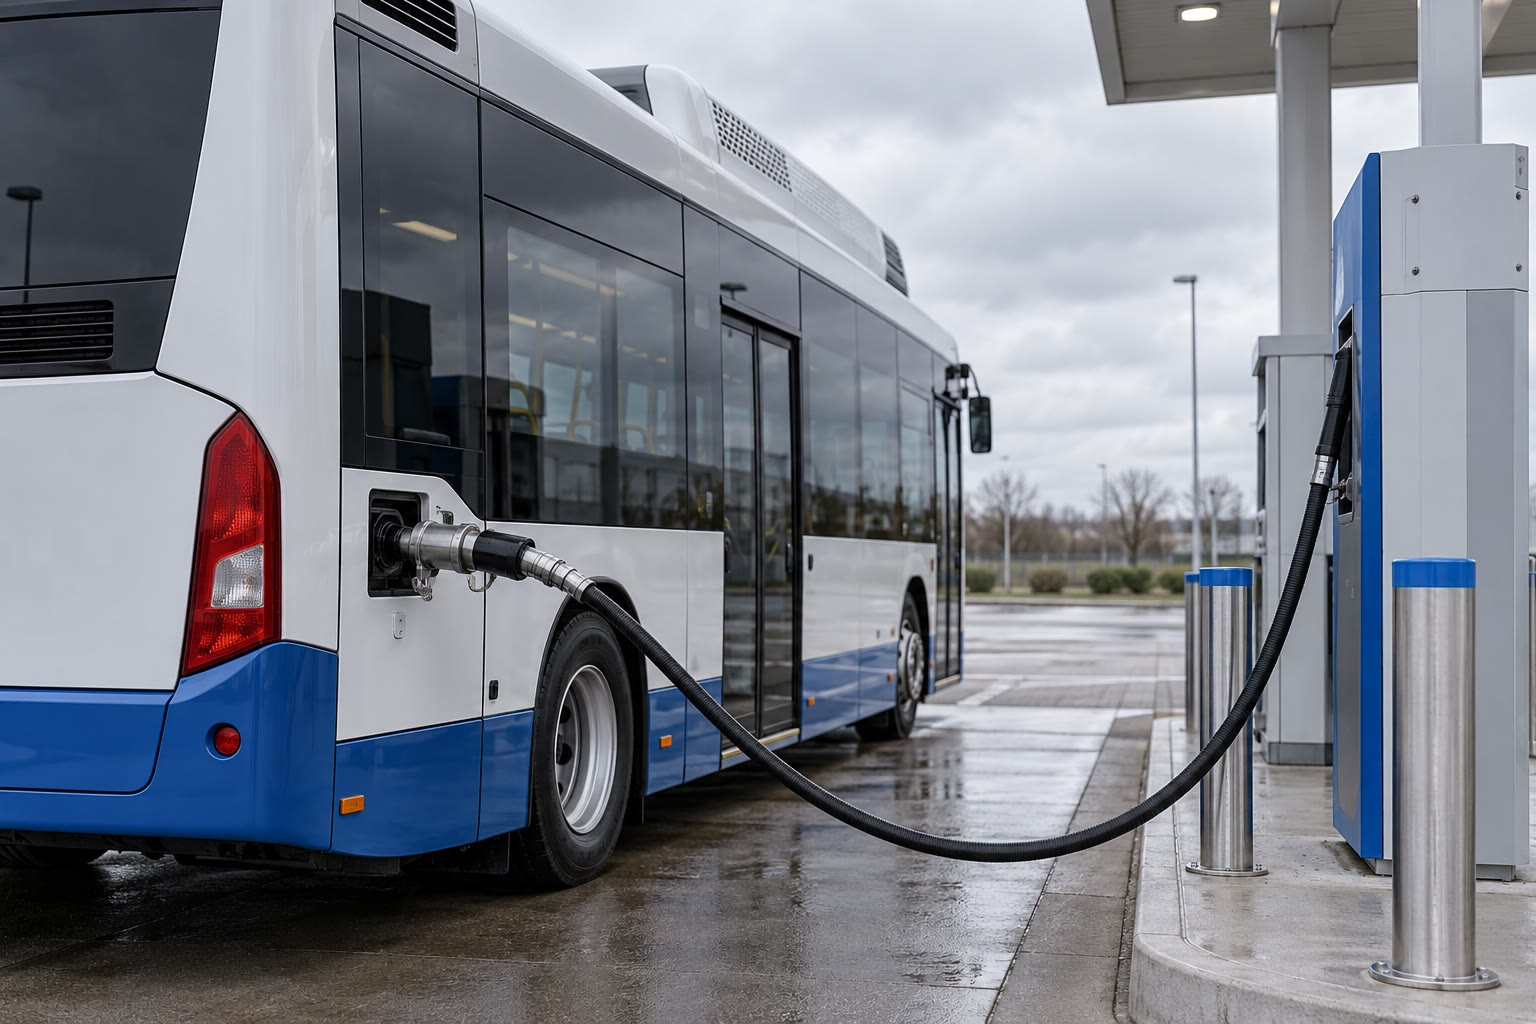
\includegraphics[width=0.5\linewidth]{images/book1/ai/g11-hydrogen-bus.jpg}

{\small Um ônibus num posto de hidrogênio: o seu \omterm{def:g4:what-a-fire-needs:fuel}{combustível} só libera
água.}
\end{omfigure}

\begin{safety}{\ghs[0.82cm]{GHS02}\ghs[0.82cm]{GHS07}}
% ledger: ghs:ethanol
O etanol é altamente inflamável e irritante para os olhos. Uma lamparina
a álcool é enchida longe de qualquer chama, nunca é reabastecida
enquanto está quente, e é usada pelo professor sobre uma placa
resistente ao calor.
\end{safety}

\section{Exercícios}


\begin{exercise}[$\star$]\label{exo:g11:reaction-energy:1}
\omterm{def:g11:reaction-energy:exothermic}{Exotérmica} ou \omterm{def:g11:reaction-energy:exothermic}{endotérmica}: a madeira queimando; o gelo derretendo; uma
compressa fria sendo apertada; um aquecedor de mãos esquentando; uma
folha verde produzindo açúcar à luz do Sol?
\end{exercise}

\begin{exercise}[$\star$]\label{exo:g11:reaction-energy:2}
% ledger: dch:CH4
Que energia libera a \omterm{def:g8:combustion-and-fuels:complete}{combustão completa} de \qty{3.0}{mol} de metano?
\end{exercise}

\begin{exercise}[$\star$]\label{exo:g11:reaction-energy:3}
No diagrama de energia de uma reação \omterm{def:g11:reaction-energy:exothermic}{exotérmica}, o que tem mais energia,
os \omterm{def:g7:chemical-reactions:reactant}{reagentes} ou os produtos? Para onde vai a diferença?
\end{exercise}

\begin{exercise}[$\star$]\label{exo:g11:reaction-energy:4}
% ledger: dch:C2H5OH
Que energia libera a \omterm{def:g8:combustion-and-fuels:complete}{combustão completa} de \qty{100}{g} de etanol?
\end{exercise}

\begin{exercise}[$\star$]\label{exo:g11:reaction-energy:5}
O que é uma \omterm{def:g11:reaction-energy:bond-energy}{energia de ligação}? Por que romper uma ligação sempre custa
energia?
\end{exercise}

\begin{exercise}[$\star\star$]\label{exo:g11:reaction-energy:6}
Estime, com as \omterm{def:g11:reaction-energy:bond-energy}{energias de ligação}, a energia da reação
\ce{2H2 + O2 -> 2H2O}, tudo no estado gasoso. Ela é \omterm{def:g11:reaction-energy:exothermic}{exotérmica}?
\end{exercise}

\begin{exercise}[$\star\star$]\label{exo:g11:reaction-energy:7}
Estime a energia da \omterm{def:g4:what-a-fire-needs:burning}{combustão} do etanol, \ce{C2H5OH + 3O2 ->
2CO2 + 3H2O}, com as \omterm{def:g11:reaction-energy:bond-energy}{energias de ligação} (desenhe primeiro a \omterm{def:g10:lewis-and-shape:lewis-structure}{estrutura
de Lewis} do etanol), e compare com o valor medido de
\qty{1367.6}{kJ/mol}.
\end{exercise}

\begin{exercise}[$\star\star$]\label{exo:g11:reaction-energy:8}
% ledger: dch:C3H8, dch:CH4
Calcule a energia liberada por quilograma de propano
(\qty{2219.2}{kJ/mol}) e de metano. Compare com o gráfico de barras.
\end{exercise}

\begin{exercise}[$\star\star$]\label{exo:g11:reaction-energy:9}
% ledger: cp:water, dch:CH4
Um fogão a gás aquece \qty{1.50}{L} de água (\qty{1500}{g}) de
\qty{15}{\celsius} até \qty{100}{\celsius}. Que energia a água recebe?
Que massa de metano é queimada se toda a energia chegar à água? E se só
metade chegar?
\end{exercise}

\begin{exercise}[$\star\star$]\label{exo:g11:reaction-energy:10}
Usando o gráfico de barras, ordene os \omterm{def:g4:what-a-fire-needs:fuel}{combustíveis} pela energia por
quilograma. Que massa de hidrogênio dá a mesma energia que
\qty{1.0}{kg} de octano?
\end{exercise}

\begin{exercise}[$\star\star$]\label{exo:g11:reaction-energy:11}
Estime a energia de \ce{N2 + 3H2 -> 2NH3}, tudo no estado gasoso.
\omterm{def:g11:reaction-energy:exothermic}{Exotérmica} ou \omterm{def:g11:reaction-energy:exothermic}{endotérmica}?
\end{exercise}

\begin{exercise}[$\star\star\star$]\label{exo:g11:reaction-energy:12}
% ledger: cp:water, dch:C2H5OH
Num experimento com lamparina a álcool, \qty{250}{g} de água esquentam
\qty{20}{\celsius} enquanto \qty{1.20}{g} de etanol queimam. Calcule a
energia recebida pela água, a energia que o etanol poderia liberar e a
eficiência do aquecimento. Dê três causas das perdas.
\end{exercise}

\begin{exercise}[$\star\star\star$]\label{exo:g11:reaction-energy:13}
% ledger: dfh:C8H18, dfh:CO2, dfh:H2O-l, dch:C3H8
O octano libera \qty{5470}{kJ/mol} e o propano \qty{2219.2}{kJ/mol}.
Escreva as suas equações de \omterm{def:g4:what-a-fire-needs:burning}{combustão} e calcule a massa de dióxido de
carbono que cada um libera por megajoule. Compare com o metano,
\qty{49.4}{g}.
\end{exercise}

\begin{exercise}[$\star\star\star$]\label{exo:g11:reaction-energy:14}
Tanto para o metano quanto para o etanol, a estimativa pelas \omterm{def:g11:reaction-energy:bond-energy}{energias de
ligação} é menor que a energia medida liberada. Dê as razões, e explique
por que a estimativa continua útil.
\end{exercise}

\begin{exercise}[$\star\star\star$]\label{exo:g11:reaction-energy:15}
Estime a energia de \ce{2H2O -> 2H2 + O2}, tudo no estado gasoso. Por
que é preciso fornecer energia (por exemplo na forma de eletricidade)
para produzir hidrogênio a partir da água? Explique por que o hidrogênio
é chamado de meio de \emph{armazenar} energia, e não de fonte de
energia.
\end{exercise}

\section{Problema: que combustível para o ônibus urbano?}

\begin{problem}[{Problema de fim de semana --- metano, etanol, octano ou
hidrogênio: qual dá mais energia por quilograma, e quanto dióxido de
carbono por megajoule?}]
\label{pb:g11:reaction-energy:1}
% ledger: dch:CH4, dch:C2H5OH, dfh:C8H18, dfh:CO2, dfh:H2O-l, be:C-H, be:OO-double, be:CO-double, be:O-H
Uma cidade compara quatro \omterm{def:g4:what-a-fire-needs:fuel}{combustíveis} para os seus ônibus: o metano (gás
natural), o etanol, o octano (pela gasolina) e o hidrogênio. As energias
liberadas pela \omterm{def:g8:combustion-and-fuels:complete}{combustão completa} de um \omterm{def:g10:the-mole:amount}{mol} são: metano
\qty{890.7}{kJ}, etanol \qty{1367.6}{kJ}, octano \qty{5470}{kJ},
hidrogênio \qty{285.8}{kJ}, com a água formada no estado líquido.

\medskip
\noindent\textbf{Parte I --- As equações de \omterm{def:g4:what-a-fire-needs:burning}{combustão}.}
\begin{enumerate}
  \item Escreva a equação da \omterm{def:g8:combustion-and-fuels:complete}{combustão completa} do metano.
  \item Do etanol, \ce{C2H6O}.
  \item Do octano, \ce{C8H18}.
  \item Do hidrogênio.
  \item Que \omterm{def:g4:what-a-fire-needs:fuel}{combustível} não libera dióxido de carbono?
\end{enumerate}

\medskip
\noindent\textbf{Parte II --- A energia por quilograma.}
\begin{enumerate}[resume]
  \item Calcule as \omterm{def:g10:the-mole:molar-mass}{massas molares} dos quatro \omterm{def:g4:what-a-fire-needs:fuel}{combustíveis}.
  \item Calcule a energia liberada por quilograma de cada um, em
        \si{MJ/kg}.
  \item Ordene os \omterm{def:g4:what-a-fire-needs:fuel}{combustíveis}.
  \item O hidrogênio ganha de longe. Por que, mesmo assim, ele é difícil
        de levar num ônibus? (Pense no seu estado à temperatura
        ambiente.)
\end{enumerate}

\medskip
\noindent\textbf{Parte III --- Estimar com as \omterm{def:g11:reaction-energy:bond-energy}{energias de ligação}.}
\begin{enumerate}[resume]
  \item Desenhe as \omterm{def:g10:lewis-and-shape:lewis-structure}{estruturas de Lewis} das \omterm{def:g7:atoms-and-molecules:molecule}{moléculas} da \omterm{def:g4:what-a-fire-needs:burning}{combustão} do
        metano, e conte as ligações rompidas e formadas.
  \item Calcule a energia necessária para romper as ligações.
  \item Calcule a energia liberada pela formação das novas ligações.
  \item Deduza a estimativa de $E_r$, e compare com o valor medido: qual
        é a diferença relativa?
  \item Dê duas razões para a diferença.
\end{enumerate}

\medskip
\noindent\textbf{Parte IV --- O dióxido de carbono por megajoule.}
\begin{enumerate}[resume]
  \item Que quantidade de metano deve queimar para liberar \qty{1}{MJ}?
  \item Que massa de dióxido de carbono ela libera?
  \item A mesma pergunta para o etanol e o octano.
  \item Que \omterm{def:g4:what-a-fire-needs:fuel}{combustível} de carbono libera menos dióxido de carbono para a
        mesma energia? Por quê (compare os números de \omterm{def:g7:atoms-and-molecules:atom}{átomos} de C e de
        H)?
  \item O hidrogênio não libera nenhum ao queimar. De que depende o seu
        verdadeiro benefício para o clima?
  \item Dê a resposta final: que massa de dióxido de carbono o metano
        libera por megajoule?
\end{enumerate}
\end{problem}
